
% This LaTeX was auto-generated from MATLAB code.
% To make changes, update the MATLAB code and republish this document.

\documentclass{article}
\usepackage{graphicx}
\usepackage{color}

\sloppy
\definecolor{lightgray}{gray}{0.5}
\setlength{\parindent}{0pt}

\begin{document}

    
    \begin{verbatim}
N1 = 48;
N2 = 36;
J1 = 0.002;
J2 = 0.0016;
c = 80;
k1 = 170;
k2 = 110;
m_a = 15;
theta2_0 = 3*2*pi/360;

num = [((N1/N2)*J2 + (N2/N1)*J1) * theta2_0, (N2/N1)*c*theta2_0 + 15];
den = [((N1/N2)*J2 + (N2/N1)*J1), (N2/N1)*c, (N1/N2)*k2 + (N2/N1)*k1];

sys = tf(num,den)

[theta2,t] = step(sys);

theta1 = (N2/N1).*theta2;

close all
plot(t,theta1)
axis([0, 2, 0, .06])
xlabel('Time [seconds]')
ylabel('\theta_1 [radians]')
box on
grid on
title('Step Response for Q7.22')
\end{verbatim}

        \color{lightgray} \begin{verbatim}
sys =
 
      0.0001902 s + 18.14
  ---------------------------
  0.003633 s^2 + 60 s + 274.2
 
Continuous-time transfer function.

\end{verbatim} \color{black}
    
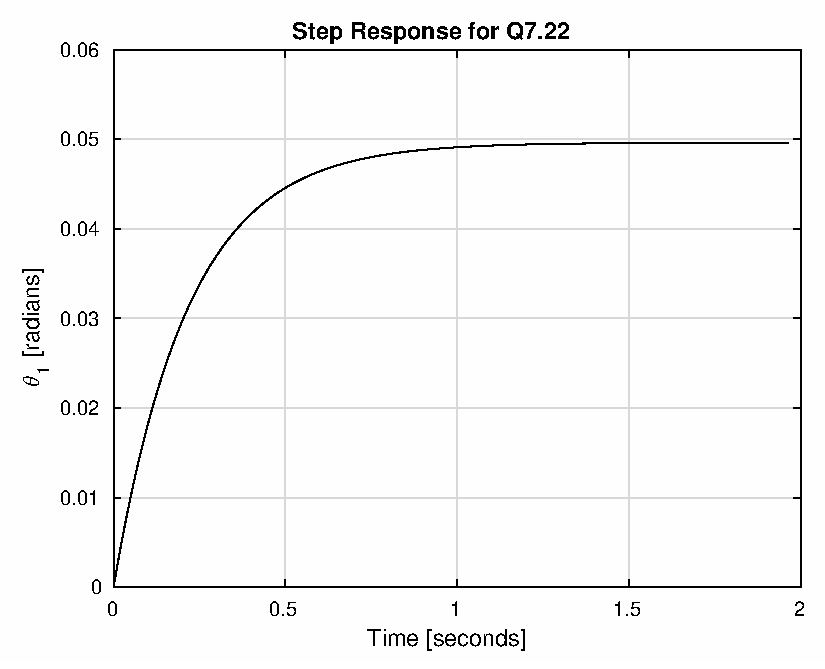
\includegraphics [width=4in]{Q7_22_01.eps}



\end{document}
    
